% This is a sample document using the University of Minnesota, Morris, Computer Science
% Senior Seminar modification of the ACM sig-alternate style. Much of this content is taken
% directly from the ACM sample document illustrating the use of the sig-alternate class. Certain
% parts that we never use have been removed to simplify the example, and a few additional
% components have been added.

% See https://github.com/UMM-CSci/Senior_seminar_templates for more info and to make
% suggestions and corrections.

\documentclass{sig-alternate}
\usepackage{color}
\usepackage[colorinlistoftodos]{todonotes}
\usepackage{comment}
\usepackage{amsmath}
\usepackage{hyperref}
\hypersetup{
    colorlinks=true,
    linkcolor=black,
    filecolor=black,      
    urlcolor=cyan,
    citecolor=black
}

%%%%% Uncomment the following line and comment out the previous one
%%%%% to remove all comments
%%%%% NOTE: comments still occupy a line even if invisible;
%%%%% Don't write them as a separate paragraph
%\newcommand{\mycomment}[1]{}

\begin{document}

% --- Author Metadata here ---
%%% REMEMBER TO CHANGE THE SEMESTER AND YEAR AS NEEDED
\conferenceinfo{UMM CSci Senior Seminar Conference, April 2019}{Morris, MN}

\title{Wing Design Using SAIL}

\numberofauthors{1}

\author{
% The command \alignauthor (no curly braces needed) should
% precede each author name, affiliation/snail-mail address and
% e-mail address. Additionally, tag each line of
% affiliation/address with \affaddr, and tag the
% e-mail address with \email.
\alignauthor
Leonid Scott\\
	\affaddr{Division of Science and Mathematics}\\
	\affaddr{University of Minnesota, Morris}\\
	\affaddr{Morris, Minnesota, USA 56267}\\
	\email{scot0530@morris.umn.edu}
}

\maketitle
\begin{abstract}
Many engineering contexts require computationally expensive models in order to learn how a design will behave.
No other domain of engineering epitomizes this struggle like the area of fluid dynamics.
If an engineer wants to know how air (or water) will move around a wing shape, they will have to use extraordinary computational power in order to simulate a wind tunnel or towing tank.
This disconnect between having a solution and knowing it's performance makes it even more difficult to try to figure out what a ``good'' design for a condition is.

To assist in this effort engineers rely on optimizers to take a solution, and tweak it until it becomes the best version of itself.
In 2014, Autodesk, a fluid dynamics model and optimizer producer, did a study(Bradner et al) to see how engineers where using their software.
They found that engineers were using Autodesk's tools in a peculiar way.
Instead of using these tools to find one excellent solution, they were using these tools to find a variety of good solutions.
By doing this, engineers could see tradeoffs inherent in the problem space, and use this information to hone in on regions of interest.
This behavior is called \textit{illumination}.

A research team from Germany and France decided to build an algorithm to illuminate problem spaces, especially when the underlying model is computationally expensive.
They called this algorithm \textit{Surrogate Assisted Illumination}, or SAIL \cite{Gaier:2018}.
We are going to walk through the SAIL algorithm, and investigate an experiment done by the authors in which SAIL is applied to the design of aerodynamic hulls for \textit{velomobiles} (very fast bicycles).
This experiment, demonstrates SAIL's potential to find a variety of high performing solutions, and an ability to teach us about the underlying model.

\begin{comment}
This paper takes a deep dive into Gaier et al's paper, \textit{Data-Efficient Design Exploration through Surrogate-Assisted Illumination}.
While many evolutionary algorithms attempt to find the optimal solution to a problem space, Gaier et al develops an evolutionary algorithm that \textit{illuminates} the problem space. 
This concept is particularly attractive in aerospace engineering as it allows engineers to properly survey the possible landscape of wing designs before investing into one particular concept heavily.

Gaier et al build off of the work of a previous algorithm called \textit{MAP-Elites}. 
MAP-Elites is designed to provide a number of high performing solutions that represent diverse regions of performance from the problem space. 
Experiments in Monet et al show MAP-Elites to be effective in creating this diverse set of solutions.
However, MAP-Elites has been shown to be extremely computationally expensive.
Moreover, MAP-Elites relies on a static model that does not change during an evolutionary run.

Gaier et al set out to improve MAP-Elites in the context of problem spaces where:
 \begin{enumerate}
   \item Running a high fidelity model is too computationally expensive to run per individual created.
   \item Running each generation comes at a significant computational cost and accuracy cost.
 \end{enumerate}
Gaier et al's algorithm, SAIL (Surrogate Assisted Illumination), uses a surrogate model to approximate the fitness of a solution instead of high fidelity model.
In its current implementation, SAIL uses a Gaussian Process as a surrogate model. In order to guess where to select new individuals, SAIL uses Bayesian Optimization (BO).
BO allows SAIL to reduce the number of generations it needs to acquire a strong, diverse set of solutions that represent a problem space well. 

This paper conducts two different experiments to test SAIL's viability in the context of aerospace engineering.
The first test attempts to design a set of two dimensional airfoils. A second test was added to design the three dimensional shape of a velomobile.
This second test was deemed important as the model to test it was much more complicated than its two dimensional counterpart.
This difficult model would stress SAIL's Surrogate Assisted model to a greater extent.
\end{comment}
\end{abstract}

\keywords{Evolutionary Computation, MAP-Elites, Gausian Processes, Bayesian Optimization}

\section{Introduction}
\label{sec:introduction}

\todo[inline]{Insert better opening statement}

Fluid dynamics stands as one of the most difficult problem spaces to model and thus design in.
The equations that govern fluid flow, known as the \textit{Navier-Stokes Equations}, are a set of of partial differential equations with no known solution.
As a result, aerospace engineers must use extraordinary computational power to approximate Navier-Stokes results.
High fidelity models of aerodynamic devices can take hours to simulate and still impart noticeable error.
Given the difficulty in modeling fluid flow, designing these devices is an extraordinary challenge.

Optimization tools aid in this challenge by helping engineers at the end of design cycle by refining a design to what is known as a local optima.
In difficult problem spaces such as fluid dynamics, there is no guarantee that an optimizer has found the best possible solution across the entire problem space.
However, the optimizer can be very confident that it has found the best solution in one small region.
We call the optimal solution across the problem space a \textit{global optima}, and an optimal solution in a subsection of the problem space a \textit{local optima}. 

In 2014, Autodesk, a producer of modelling and optimizing software found that their software was being used in a peculiar way by engineers.
Instead of using optimizing tools at the end of the design process to refine designs, engineers used them at the beginning to explore the space of possible designs (Bradner et al).
Instead of using these tools to find, with great accuracy, one local optima, they were used to find several throughout the problem space.
By finding several local optima, designers could see what tradeoffs are inherent in the problem space, and hone in on regions of interest.
This process is known as \textit{illumination}.

Over the course of several years, a research group consisting of Adam Gaier, Alexander Asteroth, and Jean-Baptiste Mouret have developed a purpose built algorithm to illuminate problem spaces, particularly when models are computationally expensive.
This algorithm, known as \textit{Surrogate-Assisted Illumination} (SAIL) uses a thus far reliable method for exploring problem spaces known as evolutionary computation, albeit in a very specialized form.
The goal of SAIL is to produce a series of high performing solutions, across the problem space, to challenging engineering problems.

\todo[inline]{Insert stuff about paper structure}

\section{Background: Evolutionary Algorithms}
\label{sec:evolutionaryAlgorithms}

SAIL uses a type of Evolutionary Algorithm to explore and exploit the problem space.
Evolutionary Algorithms (EA's) are stochastic algorithms (algorithms including randomness) inspired by biological evolution.
The premise of an Evolutionary Algorithm is that a population of potential solutions is tested against a model of the problem and assigned a \textit{fitness score}.
The individuals with the best fitness scores move onto the next generation and produce ``offspring''.
Over many generations the performance against the model will improve until either a target performance is obtained, or the algorithm reaches a fixed number of generations. 

\todo[inline]{Might include blurb about exploration vs exploitation? Will be decided after MAP-Elites section is done}

\begin{figure*}[th]
\centering
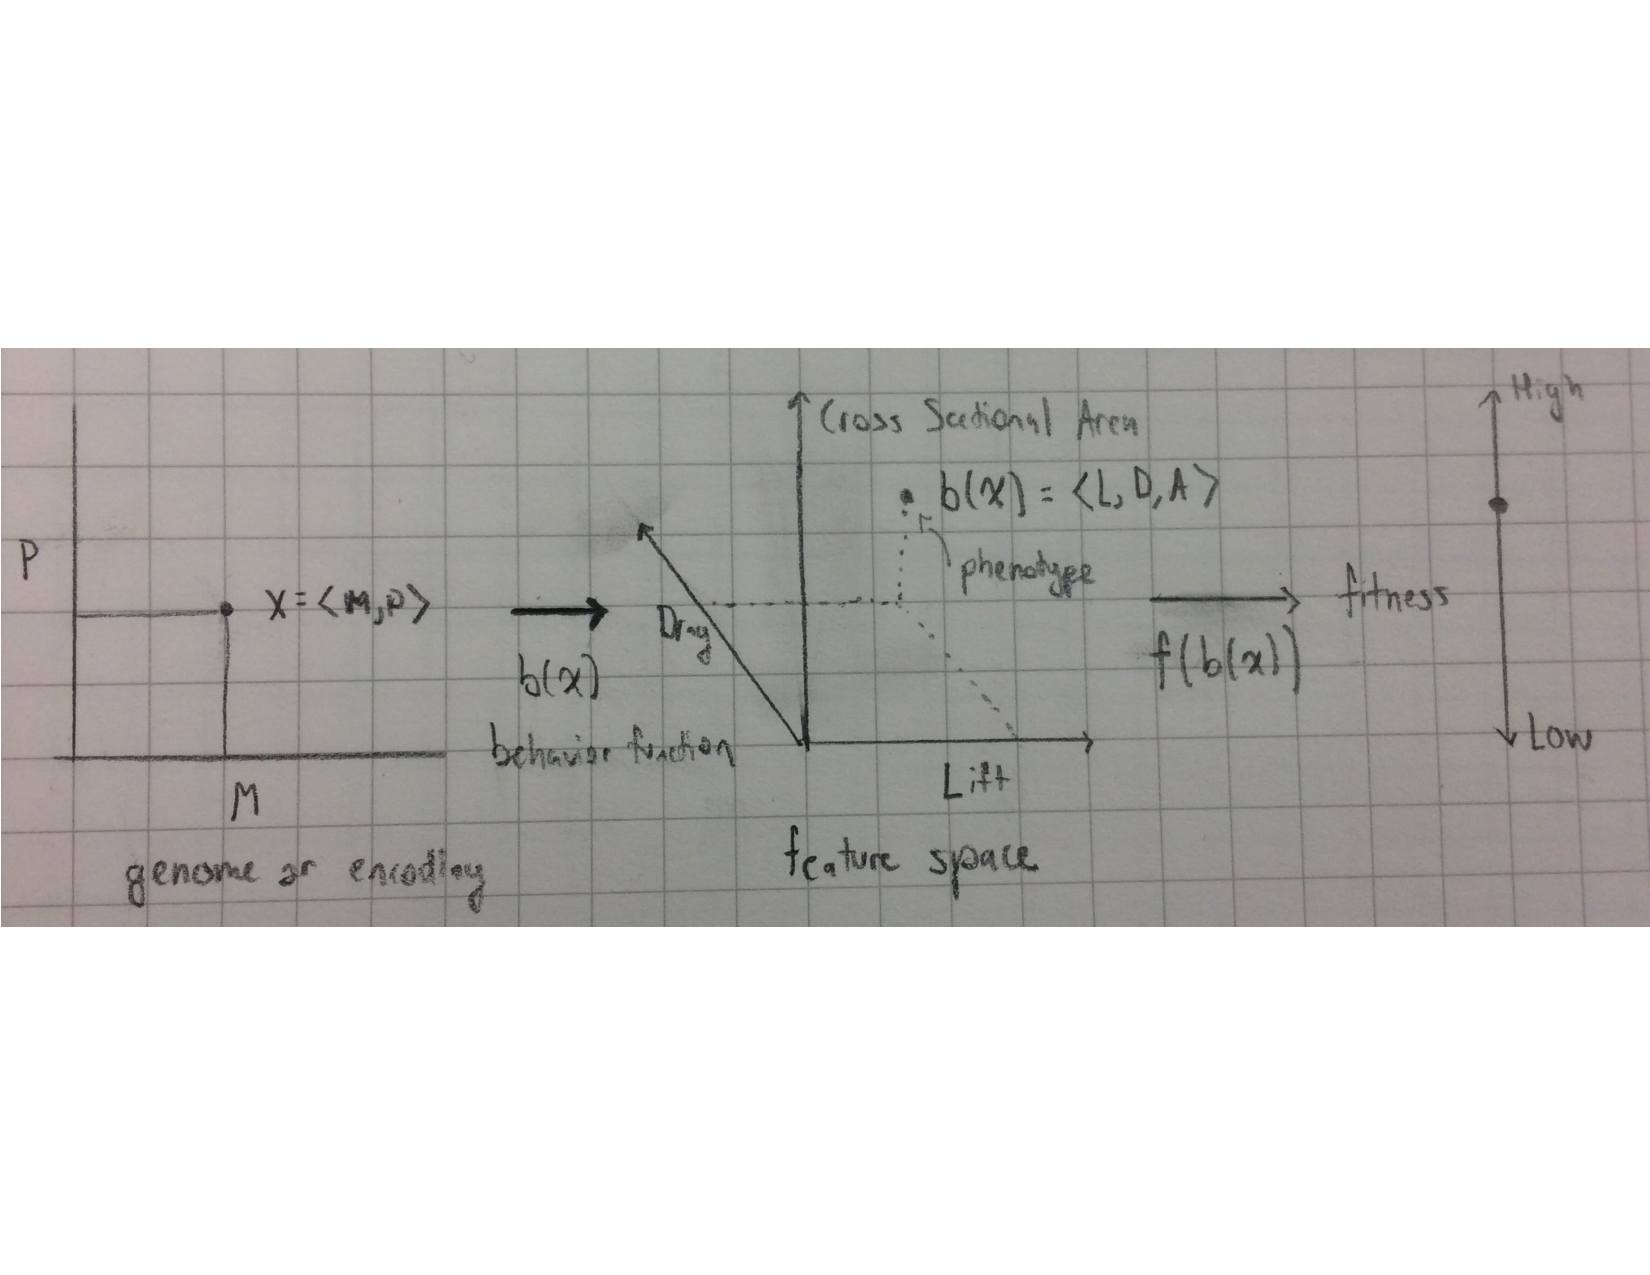
\psfig{file=genome-to-fitness.pdf,width=\textwidth}
\caption{Process of moving from an individual genome to a fitness score. \textbf{NOTE: the first space is known as the search space}}
\label{fig:genome-to-fitness}
\end{figure*}

\section{SAIL Build-up}
\label{sec:SAILBuildUp}
SAIL is made up of several components. There is:
\begin{itemize}
  \item \textbf{MAP Elites:} This is the evolutionary algorithm that SAIL is based on.
  \item \textbf{Bayesian Optimization:} The mechanism by which SAIL decides where and how new individuals will be created.
  \item \textbf{Gaussian Processes:} A way of not having to compute the expensive model by approximating it in what is known as a surrogate model.
\end{itemize}
In this section, we will go through each of these components in depth before bringing them all together and constructing Surrogate Assisted Illumination.

\subsection{MAP-Elites}
\label{sec:MAP-Elites}

MAP Elites is an Evolutionary Algorithm developed in April 2015 by Jean-Baptiste Mouret and Jeff Clune.
The purpose of MAP Elites is to \textit{illuminate} the problem space.
That is, to produce a series of high performing solutions that represent different trade offs and insights into the problem space.
Before moving into the details of MAP Elites, it is important to understand the terminology surrounding individuals in MAP Elites.

\subsubsection{Genotypes}
\label{sec:genotypes}

An important aspect in the application of any Evolutionary Algorithm is the way that individuals are represented.
In engineering contexts, there is a need to represent a physical object in all of its complexities in a compact and understandable form.
In evolutionary algorithms, this representation is referred to as an \textit{encoding} or a \textit{genotype} interchangeably.
Running with the theme of aerospace engineering, a common way to represent a two dimensional \textit{foil} (wing shape) is with a format called NACA 4 Digit Series \cite{wiki:NACAairfoil}(see fig \ref{fig:NACA4}).
NACA 4 digit foils contain three numbers refer to important geometric features about the foil shape, but also directly relate to foil performance.
We will call these values $M$, P, and T. In very rough terms, these values refer to:
\begin{itemize}
  \item M refers to how ``arched'' the foil is is.
  \item P refers to where the most ``arched'' part of the foil exists.
  \item T refers to the thickness of the foil at the most arched section.
\end{itemize}
With this compact genotype for a 2D foil, it is possible to represent a large range of complex shapes, with only three numbers.
\begin{figure}[!h]
\centering
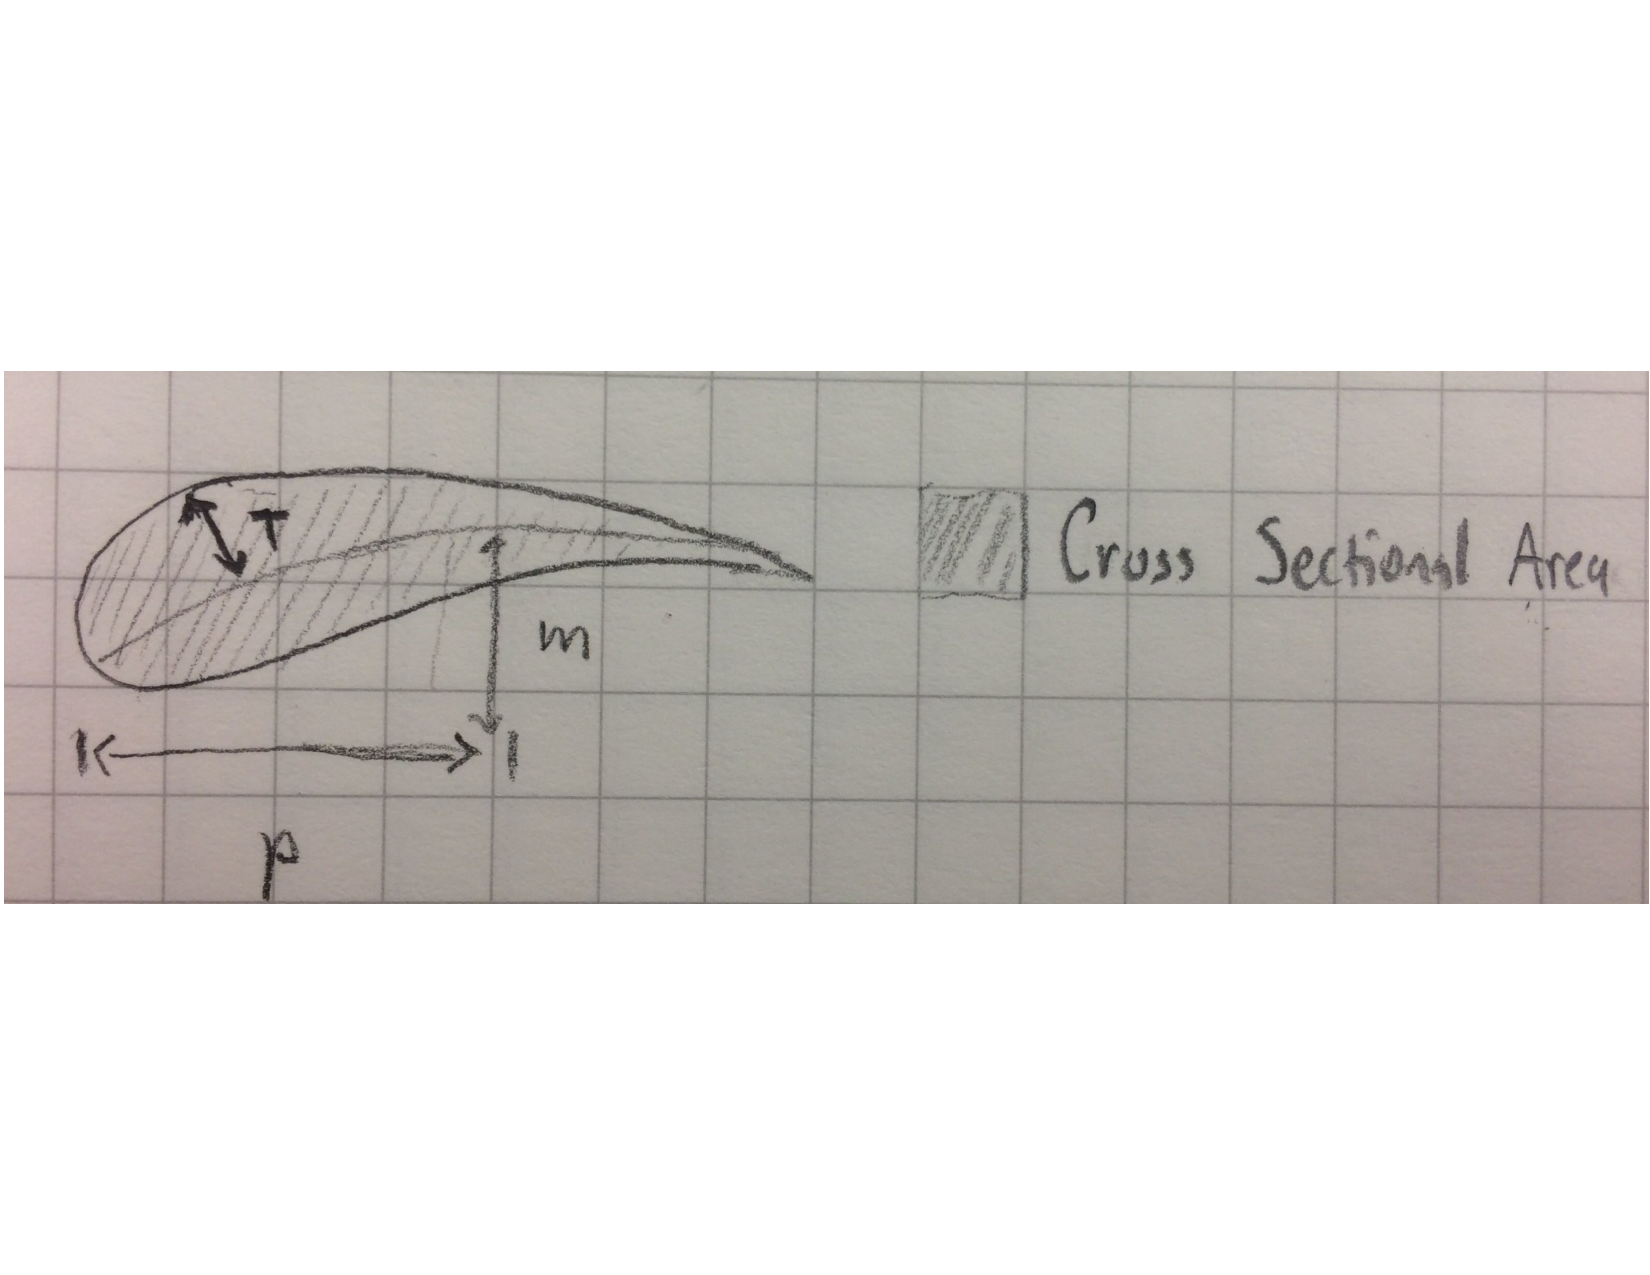
\psfig{file=NACA4-Diagram.pdf,width = 3in}
\caption{Description of NACA 4 Foil.}
\label{fig:NACA4}
\end{figure}

\subsubsection{Phenotypes}
\label{sec:phenotypes}

Once we have a representation of an individual, we can start deriving its \textit{behaviors}, or \textit{phenotypes}.
In this example, those behaviors might include the Lift and Drag of the foil in a certain condition as well as its Cross-Sectional Area.
In this case, the \textit{Feature Space}, the space of all possible phenotypes, will exist in three dimensions: Lift, Drag, and Cross-Sectional Area.
The function that takes in an individual and returns its phenotype is known as the \textit{behavior function}, denoted as $b(x)$.

\subsubsection{Fitness}
\label{sec:fitness}

MAP-Elites requires some sort of specific score so that it can strictly tell that one foil is ``better'' than another.
The \textit{fitness function} $f(x)$ takes an individual and its behaviors and returns a score quantifying how well it accomplishes our specified goals.
When developing a foil shape, we most certainly care about Lift and Drag, but for weight and structural reasons, we might also care about the foil's cross-sectional area.
A fitness function that encompasses these behaviors into a single score might look like this:
$$f(x) = a*\textit{Lift}(x) - b *Drag(x) + c*Area(x)$$
Where $a$, $b$, and $c$ are constants defined by the engineer based on which factors are more important than others.
In this example, $f(x)$ is set setup such that a \textit{higher} fitness score means a foil is better at achieving our goals, but it doesn't have to be that way.
Fitness functions can be setup such that a good score is small score, a small absolute value is a good score, etc...

\subsubsection{MAP Elites}

MAP Elites works by discretizing the feature space into a set of bins.
Each bin in the grid represents tradeoffs between features.
For example, the feature space in figure \ref{fig:FeatureSpace} is split into three sections per dimension, with three dimensions, this results in 27 bins in the feature space.
The highlighted box indicates individuals with medium lift, medium cross sectional area, and high drag.

Each generation in MAP Elites begins by creating an individual from the search space and computing its behaviors using the behavior function.
The results of the behavior function will place it in a bin of the feature space.
If there is already an individual in that bin, the fitness function will be computed on both individuals, and the individual with the superior fitness will end that generation occupying the bin.
If there is no individual in that bin, the new individual simply occupies it.

In the initial generation (generation 0), a randomly generated population of individuals is created from the search space.
Those individuals then compete for spots in the feature space.
The individuals who occupy a bin at the end of a generation are known as \textit{elites}.
During each subsequent generation, a new individual is randomly generated.
That new individual will compete with the elites from the previous generation for a bin in the feature space.

\begin{figure}[tb]
\centering
\psfig{file=DiscretizedFeatureSpace.pdf,width = 3in}
\caption{How MAP-Elites disrectizes a feature space. Here, each of three dimensions is split into three sections, yielding 27 "bins''.}
\label{fig:FeatureSpace}
\end{figure}

The default MAP-Elites pseudocode (fig \ref{fig:MAP-ElitesPCode}) creates a new individual by \textit{mutating} a random elite.
The process works as follows, an elite is randomly chosen, and then randomly ``tweaked''. 
Because small changes in the genome of an individual can result in large changes of behavior, it is common for the mutated individual to compete in a different bin than the parent.

The programmer can decide how MAP-Elites terminates.
Several options include stopping after:
\begin{itemize}
  \item A fixed number of generations is exceeded
  \item A fixed number of computational resources is exceeded
  \item The best elite has a fitness better than some threshold
  \item The average fitness of the elites is better than some threshold
  \item A certain number of bins are filled
\end{itemize}
The last point alludes to an important aspect of MAP-Elites: not all bins can always be filled.
In our example, physics does not allow a foil to have high lift, zero drag, and minimal cross-sectional area.
For this reason, the highest lift, lowest drag, lowest cross-sectional area bin might not be filled.
In addition to finding good solutions for a problem, MAP-Elites also offers insights on just where the physics of a problem caps performance of solutions.

\begin{figure*}[!t]
\centering
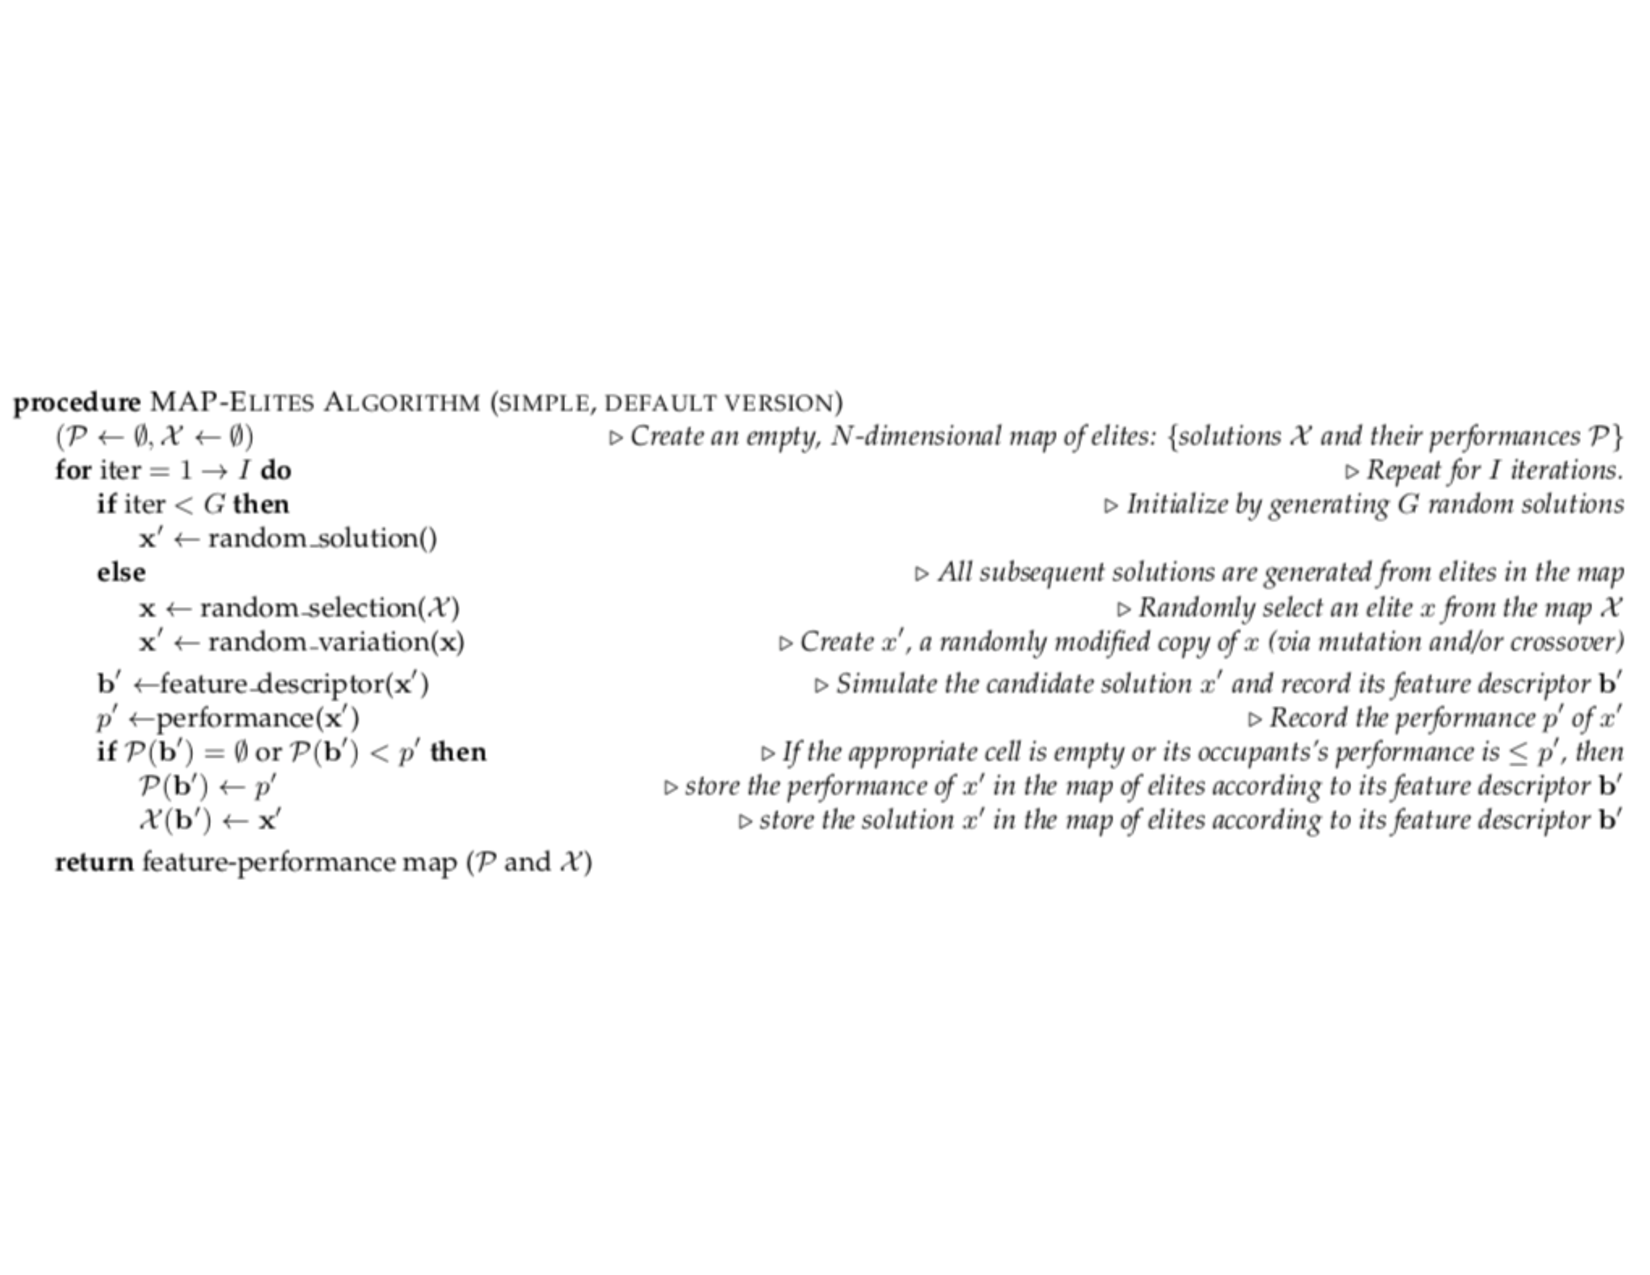
\psfig{file=MAP-ElitesAlgPCode.pdf,width = 6in}
\caption{Pseudocode of default MAP-Elites. Taken from \cite{Mouret:2015}.}
\label{fig:MAP-ElitesPCode}
\end{figure*}

\label{MAPElitesSub}

\subsection{Gaussian Process}
\label{gaussianProcess}

Like many Evolutionary Algorithms, MAP-Elites evaluates the model's fitness and behavior functions at least once every generation.
Considering a single MAP-Elites run can involve hundreds of thousands, or even millions of generations, there is a need for the model to be easy to execute.
However, in engineering contexts like fluid dynamics, computing lift and drag of a foil in high fidelity can take hours.
In cases like these, the model is prohibitively computationally expensive for use in traditional Evolutionary Algorithms

SAIL avoids computing the model directly by utilizing \textit{surrogate models} to approximate the model.
Surrogate models strategically execute the model in only limited points of the problem space. 
They then use this information to extrapolate what other parts of the model should behave like.
Gaier et al have chosen to use \textit{Gaussian processes} (GP's) as a surrogate model because they require very few queries from the model in order to start extrapolating from the problem space.
In addition, GP's include information about how confident they are about the extrapolation of a certain point in the problem space.

\subsubsection{Gaussian Distributions}
\label{GaussianDistributions}

In order to understand GP's, it is necessary to understand Gaussian distributions.
Often Gaussian distributions are also called normal distributions.
They carry the bell shape found in figure \ref{fig:UnivariateGaussian}:

\begin{figure}[htb]
\centering
\psfig{file=UnivariateGaussian.pdf,width = 3in}
\caption{Gaussian (Normal) distribution: $\mu$ is called the mean of the distribution, $\sigma$ and is called the variance.}
\label{fig:UnivariateGaussian}
\end{figure}

When a variable comes from a probability distribution, it is more likely to have a value of $x$ where $p(x)$ is high.
A variable drawn from a Gaussian distribution is most likely equal to $\mu$ (the mean).
The probability of a random variable being equal to a value $m$ from a Gaussian drops off as $m$ gets further away from $\mu$.

$\sigma$, the variance of the distribution, decides how quickly the probability drops off from the mean.
A high $\sigma$ results in a very sharp peak around $\mu$ in which a random sample from the distribution is very likely to be close to $\mu$.
A low $\mu$ results in a very flat distribution in which it is still very possible a random sample could have some distance from the mean. 

We define a Gaussian distribution as follows:

\[x ~ \sim \mathcal{N}(\mu, \sigma)\]

This is read as \textit{The random variable comes from a Gaussian distribution with mean $\mu$, and variance $\sigma$}.

\subsubsection{Multivariate Gaussian}

So far, we have described a Gaussian distribution over one variable, $x$.
However, we need to know what a Gaussian distribution looks like over many variables.
Figure \ref{fig:StandardMultivariateGaussian}, shows what a Gaussian distribution could look like over two variables, $x_{1}$ and $x_{2}$.

\begin{figure}[htb]
\centering
\psfig{file=StandardMultivariateGaussian.pdf,width = 3in}
\caption{}
\label{fig:StandardMultivariateGaussian}
\end{figure}

When we sample a point from this Gaussian, we will get a point $m$ in the $x_{1},x_{2}$ plane.
$m$ is likely to be close to our mean $(\mu_{1},\mu_{2})$.
Conversely, it will be unlikely for $m$ to be far from $(\mu_{1},\mu_{2})$.

Instead of using a single number, $\sigma$, to represent variance, the multivariate version of the Gaussian distribution uses a \textit{matrix} (a two-dimensional array),$\Sigma$, called the \textit{covariance matrix}.
In this two-dimensional case, $\Sigma$ is a two by two matrix, and each element within $\Sigma$ determines the shape of the Gaussian across the $x_{1},x_{2}$ plane.

A multivariate Gaussian is described as follows:

\[\begin{bmatrix}
    x_{1} \\
    x_{2} \\
  \end{bmatrix} 
  ~ \sim \mathcal{N}(
  \begin{bmatrix}
    \mu_{1} \\
    \mu_{2} \\
  \end{bmatrix},
  \begin{bmatrix}
    \Sigma_{11}& \Sigma_{12} \\
    \Sigma_{21}& \Sigma_{22} \\
  \end{bmatrix})\]
\[ \Vec{x} ~ \sim \mathcal{N}(\Vec{\mu}, \mathbf{\Sigma}) \]

In this representation, both the $x$'s and the $\mu$'s are written as \textit{vectors}.
Vectors are like an array in which each element represents a different axis of the space.
We can collapse this representation with with second notation.

This description is read as \textit{the vector $\Vec{x}$ comes from a multivariate Gaussian with mean $\Vec{\mu}$ and covariance matrix $\mathbf{\Sigma}$.}

\subsubsection{Gaussian Regression: Training the Model}

The goal of a Gaussian Process is to fit a multivariate Gaussian to a set of observations about the underlying problem space.
We call this process regression.
Let's imagine we have an unknown function $f(x)$, we will try to build a Gaussian to fit this function with Gaussian regression (See figure \ref{fig:GPRegression}).

\begin{figure}[htb]
\centering
\psfig{file=GPRegression.pdf,width = 3in}
\caption{}
\label{fig:GPRegression}
\end{figure}

In this example, the multivariate Gaussian that models these points will be a Gaussian of three variables (one for each observed point).
In any Gaussian regression, this Gaussian will have 0 mean.
In order to shape this Gaussian to fit our data well, we need to introduce a kernel matrix, \textit{K}.
Ultimately, we decide the values for each element in K.
The rule that we use to define these values in known as the \textit{kernel}.
In Gaussian processes, it is common to use the \textit{squared exponential kernel}:

\[k_{i,j} = e^{-\|x_{i} - x_{j} \|^{2}} = 
    \begin{cases} 
      0 & \|x_{i} - x_{j} \| \rightarrow \infty\\
      1 & x_{i} = x_{j}
    \end{cases}\]
    
As the distance between x's decrease, the squared exponential kernel will get closer and closer to one.
As distance between x's increase, the squared exponential kernel will drop off exponentially towards 0.
The idea behind the squared exponential kernel is that small changes in x, will result in small changes to $f(x)$. A squared exponential kernel will result in a smooth transition from one observed point to another. 

\subsubsection{Gaussian Processes: Extrapolating Points}

Via Gaussian regression, we have fit a multivariate Gaussian to our observed data from the problem space.
Now, we want to predict what $f(x)$ will be for values of x not in our observed data.
In the following case, we want to find $f_{*}$ for a given $x_{*}$ (See \ref{fig:GPEXT}).

\begin{figure}[htb]
\centering
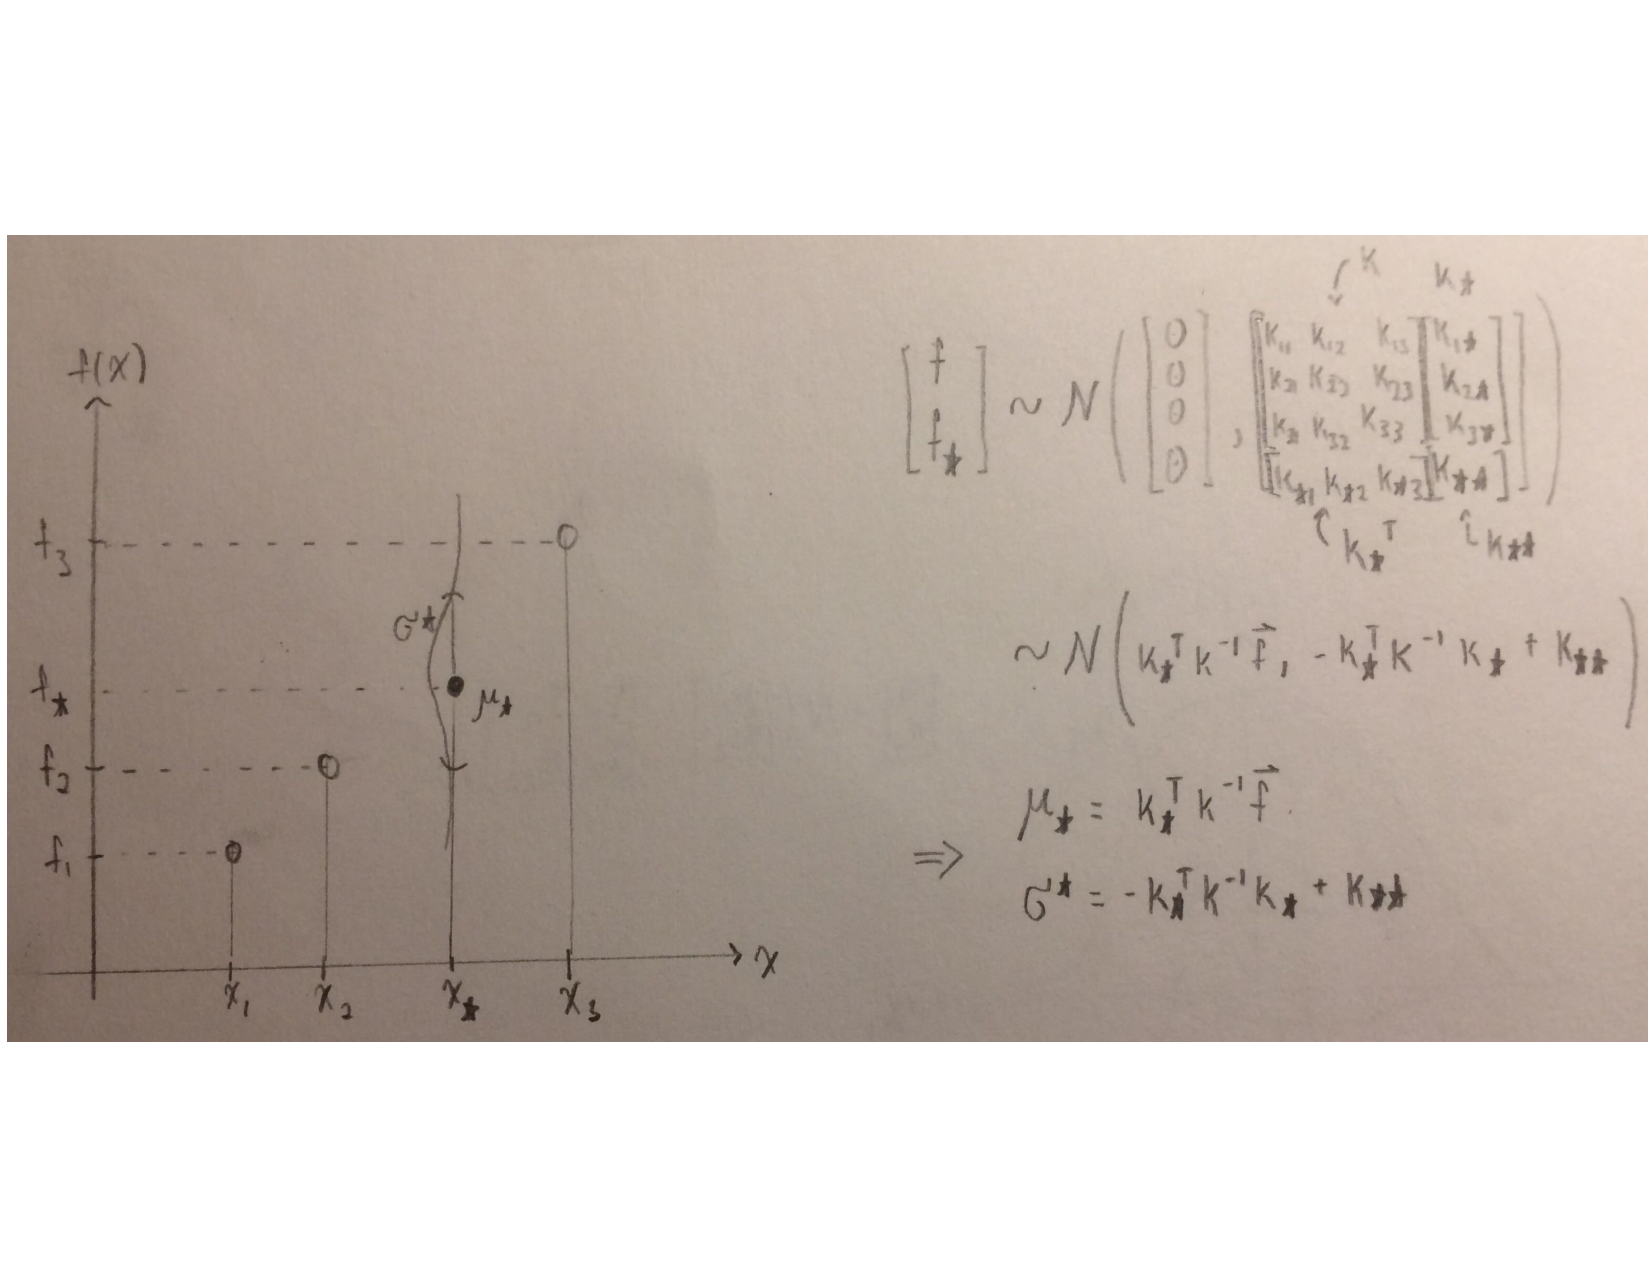
\psfig{file=GP_EXT.pdf,width = 3in}
\caption{}
\label{fig:GPEXT}
\end{figure}

We extrapolate $f_{*}$ by creating a new Gaussian via \textit{appending} $f_{*}$ to our Gaussian from the Gaussian regression.
This new Gaussian will have four variables that will range from $f_{1}$ to $f_{3}$ (our training set $f$), and $f_{*}$.
Just like before, this new Gaussian will have 0 mean for each variable.
However, we now have to compute the kernel to and from each point in our training set and $x_{*}$.
Figure \ref{fig:GPEXT} shows how the kernel from this new Gaussian can be segmented into four pieces:

 \begin{itemize}
   \item Our $\mathbf{K}$ from the training set.
   \item $\mathbf{K_{*}}$, the kernel from each point in the training set to $x_{*}$.
   \item $\mathbf{K_{*T}}$ (Read as $\mathbf{K_{*}}$ transpose), the kernel from $x_{*}$ to each point in the training set.
   \item $\mathbf{K_{**}}$, the kernel of $x_{*}$ to itself.
 \end{itemize}
 
 It is possible for this new Gaussian to be written as follows.
 However, the proof for this is outside the scope of this paper.
 
\[\begin{bmatrix}
    f \\
    f_{*} \\
  \end{bmatrix} 
  ~ \sim \mathcal{N}(
    ,\mathbf{K_{*}^{T} K^{-1}} \Vec{f}
    -\mathbf{K_{*}^{T} K^{-1} K_{*}} + \mathbf{K_{**}} )\]
    
\footnote{This notation features several concepts from linear algebra.
First the processes of matrix/vector multiplication, and the \textit{inversion} ($\mathbf{K}^{-1}$) of a matrix.
While these concepts are straightforward, space constraints prevent us from discussing them in depth. If you are interested in learning about matrix multiplication, please see \url{https://youtu.be/aKhhYguY0DQ}.
If you are interested in learning about matrix inversion, please see \url{https://youtu.be/iUQR0enP7RQ}.}

This new representation allows us to say that $f_{*}$ is a Gaussian with mean and variance:

\[ \mu_{*} \sim \mathbf{K_{*}^{T} K^{-1}} \Vec{f},  \sigma_{*} \sim  -\mathbf{K_{*}^{T} K^{-1} K_{*}} + \mathbf{K_{**}}\]

Looking at figure \ref{fig:GPEXT}, we can see that our approximation for $f_{*}$ is simply the mean, $\mu_{*}$, and our confidence in this prediction is marked by our variance, $\sigma_{*}$.

If we can extrapolate $x_{*}$, we can extrapolate a different $x_{*2}$ not in the training set.
We simply append this new $f_{*2}$ to our training set $f$, and arrive at a four dimensional Gaussian.
We take the mean and variance from this Gaussian and plot it just as we did for $x_{*}$.

If we extrapolate so many points that to the human eye, the means and variances form lines, and we can see the full result of our Gaussian process in figure \ref{fig:GP-Complete}.

\begin{figure}[htb]
\centering
\psfig{file=GP-Complete.pdf,width = 3in}
\caption{}
\label{fig:GP-Complete}
\end{figure}

Using the squared exponential kernel, we get a smooth mean prediction.
More importantly, we can measure how confident each prediction is at every single point.
The variance contracts around our observed points, and expands as we get farther away from the observed points.
This leads to an important feature of Gaussian processes: \textit{Where there is data, we are confident, where there is no data, we are less confident}.

\subsection{Bayesian Optimization}
\label{bayesianOptimization}

The fact that Gaussian processes are confident where there is data, and less confident where there is not, allows us to ask an important question:
\textit{If we were to add another point to our Gaussian processes, where would we do it?}
If our objective is to maximize the function modeled by our Gaussian processes in Figure \ref{fig:GP-Complete}, then our new point can help us do that in one of two ways:
First, we could try to pick a point where our prediction is maximized, very near $x_3$; this is called \textit{exploiting} our problem space.
Second, there is an area in between $x_2$ and $x_3$ in where the model has a high variance.
Selecting a point in this area would improve the overall accuracy of our model, and there might just be a maxima to the function in that region.
Selecting a point for this rational is called \textit{exploring} the problem space.

The degree to which we should explore or exploit the problem space is a difficult question;
\textit{Bayesian Optimization} attempts to provides a solution.

\begin{figure}[htb]
\centering
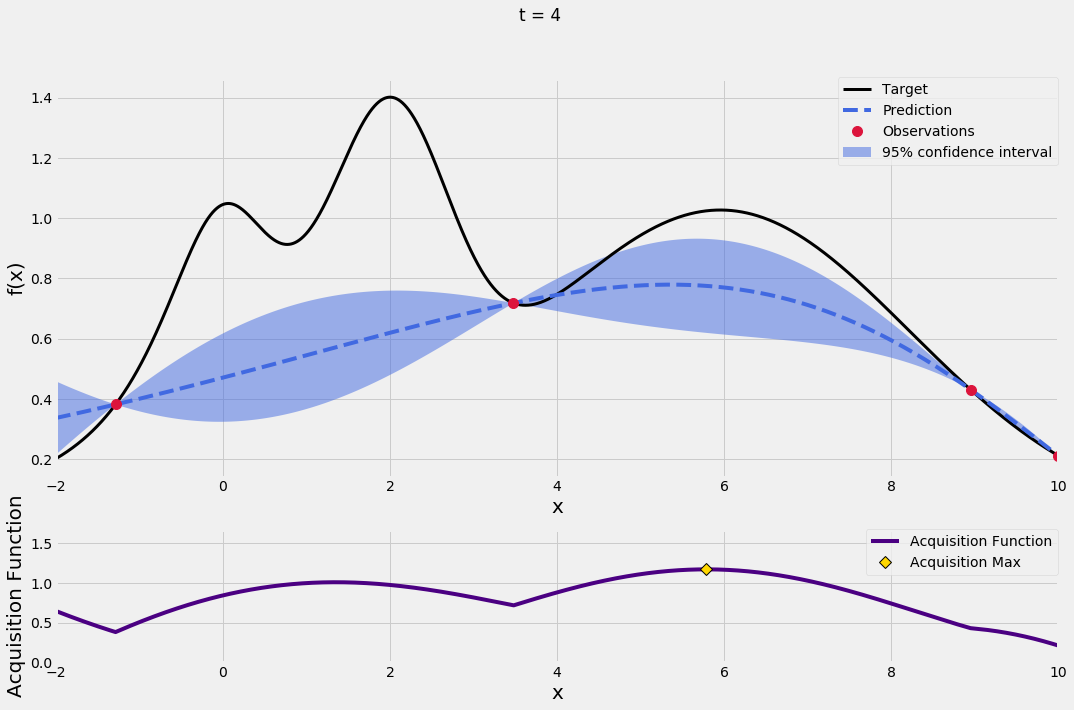
\psfig{file=t-4.png,width = 3in}
\label{fig:t4}
\end{figure}

\begin{figure}[htb]
\centering
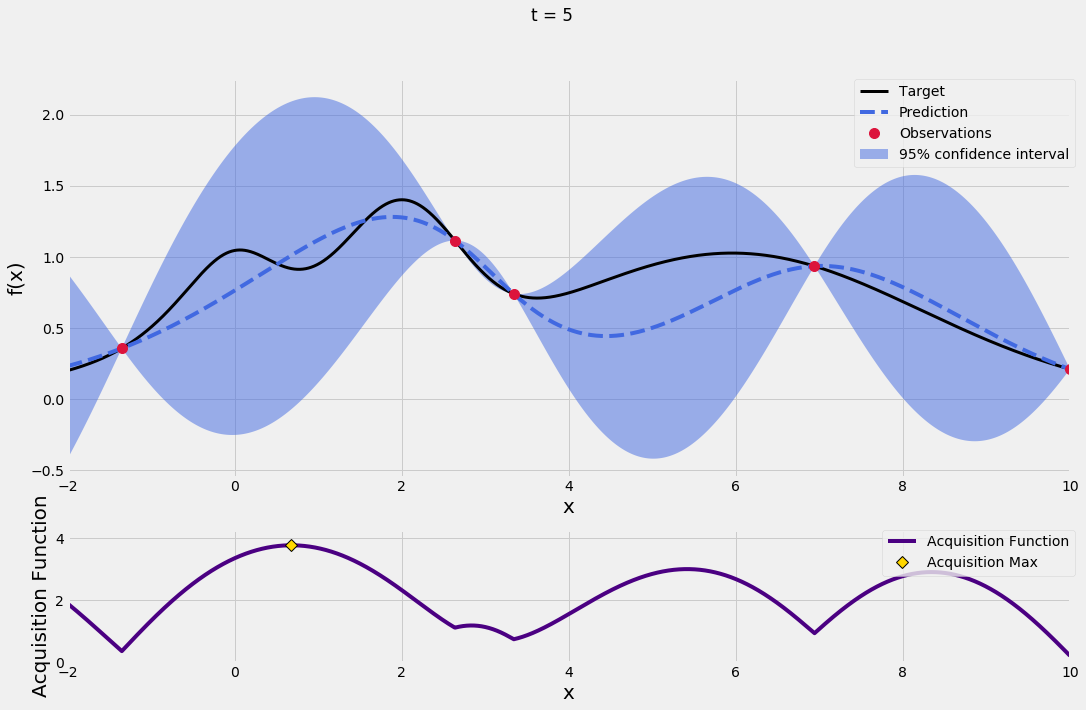
\psfig{file=t-5.png,width = 3in}
\label{fig:BO5}
\caption{}
\end{figure}

Bayesian Optimization provides a rule for computing the \textit{utility} of observing another point.
There are many different ways of computing utility with Bayesian Optimization;
Gair et al decided to use the \textit{Upper Confidence Bound Optimizer}:

\[ UCB(x) = \mu(x) + k\sigma(x) \]

The utility of observing a new value from the model, the $UCB(x)$, is the linear combination of the the mean prediction at a point, $\mu(x)$, and some constant $k$, times the variance, $\sigma(x)$, at some point.
Varying $k$ tunes the model to favor exploration vs exploitation in different quantities. We call the resulting function the \textit{acquisition function}.

Figure \ref{fig:BO5} shows how a Bayesian Optimization is applied to a Gaussian Processes.
The black line represents the underlying function we are trying model, the blue dotted line represents the mean estimation from the Gaussian processes, and the blue shaded region shows the confidence bounds for the GP.
Below, the UCB is computed along the x axis.

The left side shows the GP with four observations (There is a red dot very far on the right).
At this stage, the model is not doing too well at approximating the true function.
Maximizing the acquisition function gives us a point with both a high approximated value and a high variance.

We select that point, re-compute the Gaussian processes and rebuild the acquisition function.
The updated GP and acquisition function is shown on the right.
Again, UCB balances exploration vs exploitation and finds a point with a high predicted value, and high certainty.
Using Bayesian Optimization allows the GP to model the underlying function with very few points, and make significant progress with each observation. 

\subsection{SAIL Algorithm}
\label{SAILAlgorithm}

Understanding Gaussian processes and Bayesian Optimization allows us to construct Surrogate Assisted Illumination (SAIL).
The pseudocode of SAIL is shown in figure \ref{fig:SAILpcode}.
SAIL consists of three phases: 
1) Creation of the Gaussian processes, 
2) The production of the acquisition map, 
3) The production of the prediction map. 

\begin{figure}[htb]
\centering
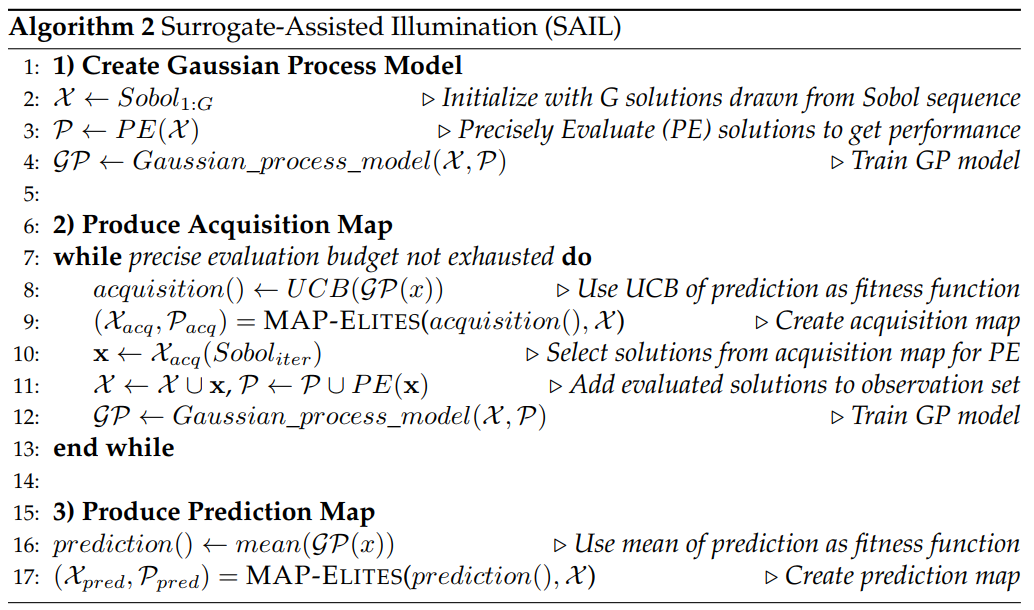
\psfig{file=SAILpcode.PNG,width = 4in}
\label{fig:SAILpcode}
\caption{}
\end{figure}

The first stage of the algorithm consists of sampling the problem space and building a Gaussian processes.
Recalling the foil terminology used in section 3.1, SAIL would create random individuals with \textit{M} and \textit{P} values, compute the precise model for each of them, and use those results to build a Gaussian process.
The random solutions are created using a random number generator called a Sobol sequence.

Next, SAIL trains the Gaussian processes by producing an \textit{acquisition map}.
In this stage, an acquisition function is computed from the Gaussian process using the \textit{Upper Confidence Bound} (UCB).
It is important to note that even though the UCB acquisition function may be made up of a linear combination of components, these components are in no way simple shapes.
For this reason, the acquisition function will not have intuitive shapes.
Moreover, in problems where a individual is comprised of many genomes, the acquisition function may be a high dimensional shape (ex: 5 dimensions).
Considering this, finding optima in the acquisition function can become a challenge.
MAP-Elites is perfectly suited to find not just the global optima of the acquisition function, but illuminate the acquisition function.
The resulting set of high utility individuals is called the \textit{acquisition map}. 

SAIL takes a random set of individuals from the acquisition map, and runs the computationally expensive model on them.
Now there is a larger set of observed values that can be used to retrain the Gaussian processes.
The loop will enter its next iteration, it will repeat the process of creating the acquisition function, illuminating the acquisition function to create an acquisition map, selecting individuals from the acquisition map for precise evaluation, and rebuilding the Gaussian process with the new observations.
This processes will continue until a fixed computational budget is reached.

Through extensive iteration, the Gaussian process ossifies into a robust model that accurately describes the underlying function.
The goal of SAIL is to illuminate the underlying function.
This task is fulfilled by illuminating the mean prediction of the Gaussian processes using MAP Elites.
The result of this illumination is a set of well performing solutions describing the various optima of the problem space.
We call this result set of solutions the prediction map.

\section{3D Foil Experiment: Velomobile Experiment}
\label{3DFoilExperiment}

Gaier et al included two experiments in their paper.
Due to space constraints, we will only visit the more ambitious of the two:
The application of SAIL to design three dimensional shapes of aerodynamic hulls for \textit{velomobiles}.
Velomobiles, shown in figure \ref{fig:Velomobile}, are fully human powered "bicycles".
The cyclists in a velomobile sit in a \textit{recumbent position}, like one would sit in a paddle boat, and are enclosed in an aerodynamic hull.
This design allows the center of gravity of the velomobile to low in comparison to a bicycle, and the hull allows engineers to carefully craft the airflow around the velomobile to reduce drag.
Velomobiles hold several world speed records for human powered devices.

\begin{figure}[htb]
\centering
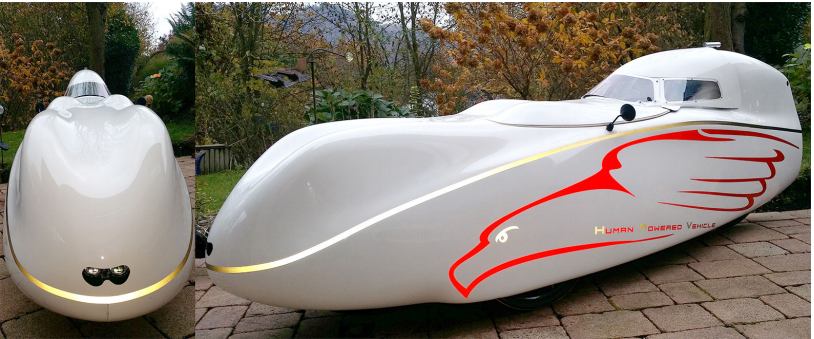
\psfig{file=Velomobile.PNG,width = 3in}
\label{fig:Velomobile}
\caption{}
\end{figure}

As seen in figure \ref{fig:Velomobile}, velomobiles have unintuitive hull shapes.
The strange contours to these hulls provide an interesting problem space to illuminate.
Moreover, the fluid dynamics software that simulates how air moves around the hull shape has high computational cost, stressing the need for a \textit{data efficient} approach to illumination.
In short, the illumination of velomobile hulls is a good testing ground for SAIL.

Gaier et al encountered several difficulties with this experiment.
Most prevalently, the data efficient nature of this problem rules out use of two other control techniques for illumination:
MAP-Elites, and another optimizer called CMA-ES.
With these technique's heavy reliance on the computationally expensive model, illuminating these shapes would take hundreds, if not thousands of hours to run.
Previous experiments in \cite{Gaier:2018} demonstrate SAIL's ability to create near optimal solutions in fluid dynamic contexts, so the focus shifted from testing SAIL's ability to compete against other illumination algorithms, to focusing on how different velomobile representations affect performance of the SAIL algorithm.
Two representations, or encodings, of velomobile shape, are used in this experiment: a parameterized, and deformed encoding.

\subsection{Parameterized Encodings}
The parameterized encoding uses a set of aerofoil shapes to create a three dimensional velomobile hull as seen in figure \ref{fig:ParameterizedEncoding}.

\begin{figure}[htb]
\centering
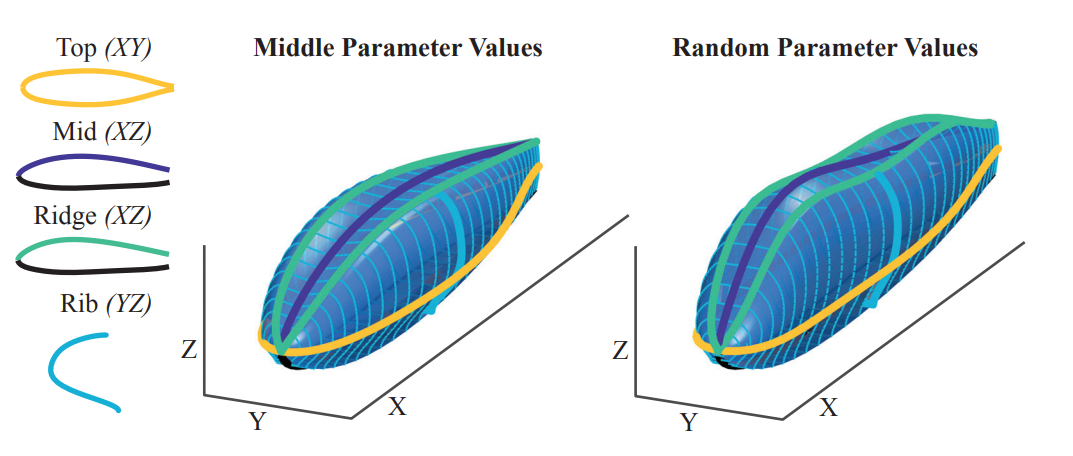
\psfig{file=ParameterizedEncoding.PNG,width = 3in}
\label{fig:ParameterizedEncoding}
\caption{}
\end{figure}

There are four foil shapes in the parameterized encoding.
The top foil shape, is a symmetrical foil that defines the hull at its widest point from above.
The mid foil shape represents the foil at it's centerline.
The ridge foil represents the hull where the cyclists knees protrude upward.
Finally, the rib foil effects how aggressively curved surface of the hull will be in order to cross through these foils correctly.
All in all, this encoding will contain 16 parameters that affect hull shape. 
An advantage of an encoding like this is that each of the 16 parameters are known to change the aerodynamic properties of their respective foil shape.

\subsection{Deformation Encodings}
Where the parameterized encoding SAIL to change key aspects of the shape directly corresponding to performance, deformed encodings take the opposite approach.
Deformation encodings try to ``decouple the complexity of a the design from the complexity of the representation''.
That is, deformed representations allow SAIL to find key features of foil performance on its own.
Figure \ref{fig:Deformation} shows an example of a deformation encoding:

\begin{figure}[htb]
\centering
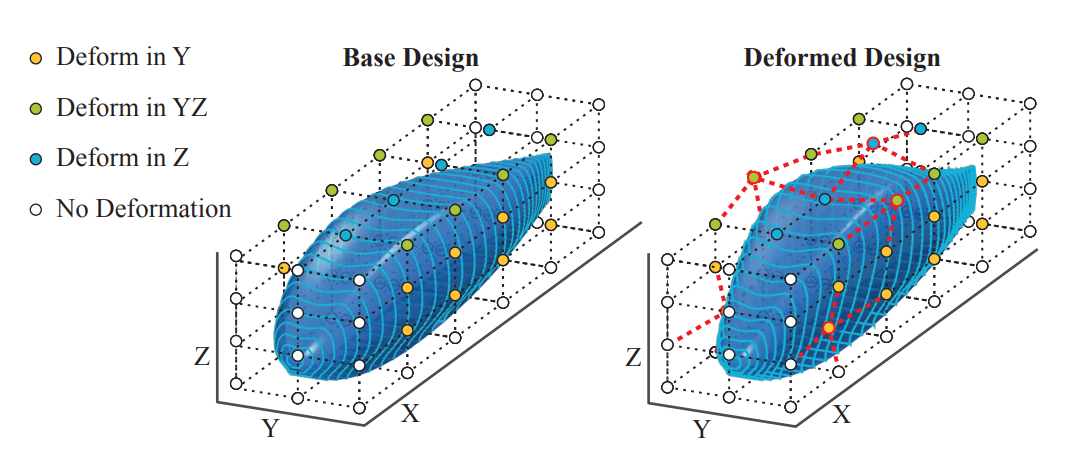
\psfig{file=Deformation.PNG,width = 3in}
\label{fig:Deformation}
\caption{}
\end{figure}

Deformation encodings start with a base design, and surround it with a \textit{lattice}, or grid, of \textit{control points}.
These control points can be shifted in a particular axis.
As a control point is moved, the base design will \textit{deform} to adjust to the shifted control point.
This particular representation allows for 16 different points to be altered, each in only one axis.

\subsection{Experimental Setup}
The goal of this experiment is to see how two features, curvature and volume impact the drag of a velomobile shape.
It is known that an increase in volume of a shape leads to an increase in drag, but a designer might want to have explored how volume impacts drag to accommodate shifting requirements about the volume (all of a sudden, the pedaling mechanism might need to take up more space).
Moreover, designs with less curvature will generally have less drag, but the thin carbon fiber might might require additional (heavy) reinforcement to prevent flutter at high speed. 

SAIL will start with 200 velomobile shapes to train the GP model. During each iteration of the illumination phase, 10 individuals will be chosen from the acquisition map to improve the GP.
There will be a total of 100 illumination iterations leading to 1000 precise evaluations during the illumination phase.
The feature map will be discretized into a 25 x 25 map, leading to 625 bins. 

Fitness will be computed as the drag force on the velomobile as it travels at 20 m/s (44.7 mph).
A low drag force will represent a better velomobile.

\subsection{Results: Design Performance}
The following diagram shows the prediction maps for both the deformed and parameterized encodings as well as a comparison against the two.
In the left two images, a lighter colour indicates more drag, and a cooler colour indicating less.
In this experiment, we are aiming to minimize drag, so darker regions are preferred.

\begin{figure}[htb]
\centering
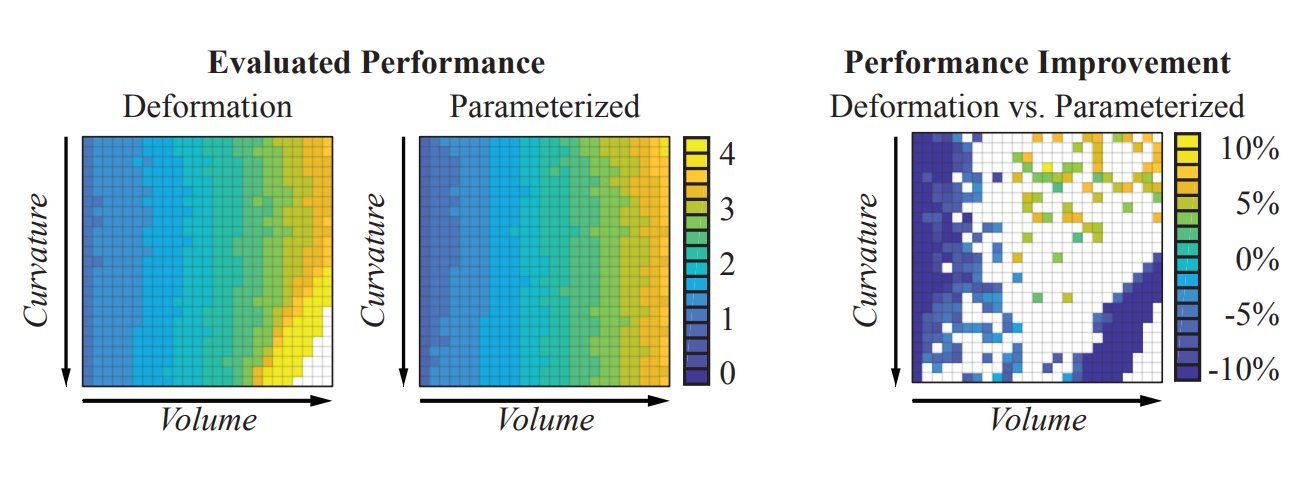
\psfig{file=DesignPerformance.png,width = 3in}
\label{fig:DesignPerformance}
\caption{}
\end{figure}

It's apparent that the deformation encoding has a set of empty bins in the high volume, high curvature section of its prediction map.
This is because the deformed encoding is too tightly constrained to create high volume, high curvature solutions.
It is clear that drag does increase as volume increases.
However, it seems that encoding constraints aside, curvature does not seem to have a strong impact on drag.

The right side of figure \ref{fig:DesignPerformance} shows the deformation encodings' successes against the parameterized encoding.
Lighter colour highlights regions where deformation has a better fitness than the parameterized encoding;
Cooler colour indicates the converse.
There is only colour where there is a significant change in fitness between the two encodings.
Deformation does better in the high volume, low curvature region of the feature space, where as the parameterized encoding does better around the edges of the feature space.

\subsection{Results: Model Accuracy}
After each SAIL run, every individual in the prediction map was tested against the computationally expensive model in order to record errors in the GP model at the end of the run.

\begin{figure}[htb]
\centering
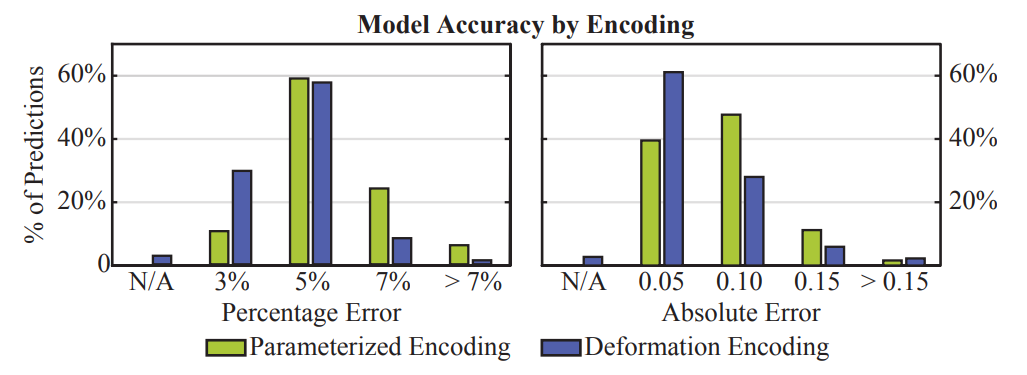
\psfig{file=ModelAccuracy.PNG,width = 3in}
\label{fig:ModelAccuracy}
\caption{}
\end{figure}

Figure \ref{fig:ModelAccuracy} shows that roughly 60\% of the drag calculations for individual's where within 5\% of the computationally expensive fluid dynamics model.
The parameterized encoding was within 0.1N of the true drag value roughly 50\% of the time.
The deformed encoding was within 0.05N of the true drag value over 60\%.
It is unclear why the deformed encoding would have a lower error than the parameterized model.

\subsection{Results: Design Exploration}
The two encodings lead to very different looking solutions that occupy the same bins in the prediction map at the end of the SAIL run.
Figure \ref{fig:CrossSections} shows various cross sections of the deformed and parameterized solutions across several bins.
For nearly all of these cross sections, the parameterized solution is taller than its deformation equivalent. 

\begin{figure}[htb]
\centering
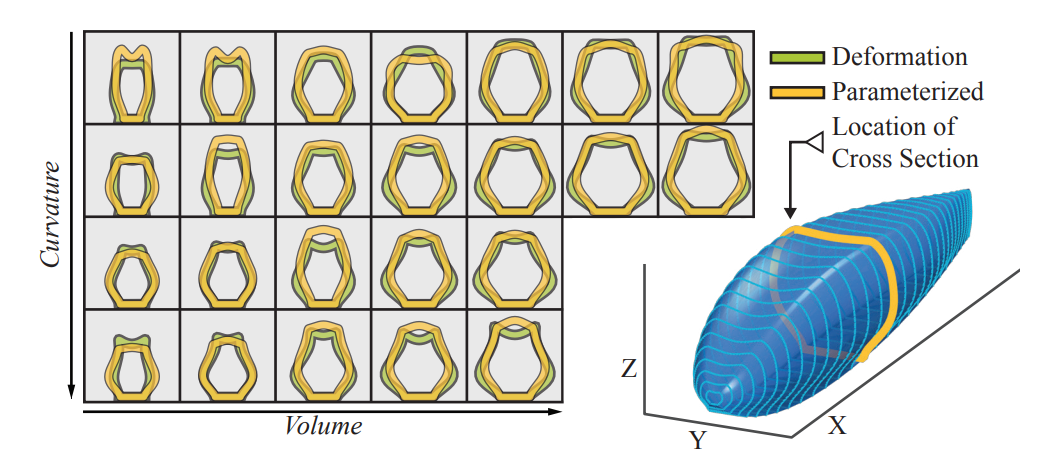
\psfig{file=CrossSections.PNG,width = 3in}
\label{fig:CrossSections}
\caption{}
\end{figure}

Gaier et al suspect that parameterized encodings are taller than deformed encodings because they have more freedom to pinch the nose of the velomobile than deformed encodings can (see figure \ref{fig:3DShapes}).
A pinched nose reduces frontal area, thereby reducing pressure on the nose of the velomobile.
While deformed designs lack this geometric freedom, they make up for it by smoothing out the shape along the length of the entire velomobile, especially where the knee ridges meet the rest of the hull.

\begin{figure}[htb]
\centering
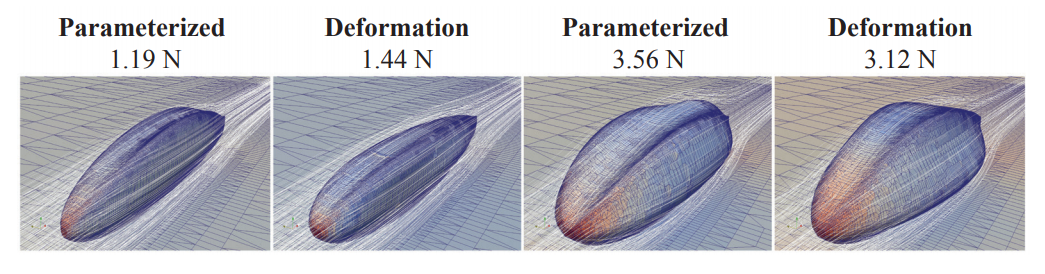
\psfig{file=3DShapes.PNG,width = 3in}
\label{fig:3DShapes}
\caption{Two sets of similarly performing solutions that highlights the geometric tendencies of each encoding.
The left side includes two similarly performing low volume velombiles.
The right includes two similar high volume designs.
The red indicates how aerodynamic pressure is distributed over the velomobile shape.
Areas of greater intensity of red indicate higher aerodynamic pressure.}
\end{figure}

These experiments show how various encodings can reach similarly performing solutions from different directions.
Moreover, these experiments showcase SAIL's ability to create a variety of high performing solutions independent of encoding.

\section{Conclusions}
\label{sec:conclusions}
The velomobile experiment has demonstrated several qualities and observations about SAIL’s capabilities.
These velomobile experiments show the potential of SAIL as a powerful algorithm for illuminating problem spaces in computationally difficult problem spaces.
Moreover, SAIL could be used for testing the limits of various encodings of individuals.
Before, committing to a specific encoding, SAIL can show whether or not that encoding is capable of reaching far areas of the feature space.
Moreover, SAIL can give an engineer insights as to how each individual point of variation in the encoding contributes to the performance. 

A particular advantage of SAIL is that it doesn’t just have to return a set of high performing solutions, but also the final GP model.
This model can be used to gain insights on the problem space.

Gaier et al mention that a potential bottleneck for SAIL is the behavior function.
For example, in the 2D foil example of MAP-Elites, the features include lift, drag, and cross sectional area.
Even though the fitness function is not hard to compute, the behavior function will take a large amount of computational energy to compute lift and drag.
Gaier et al propose the expanded use of surrogate models in the behavior function in cases where the behavior function is too computationally expensive to run for every individual in a SAIL run.

\section*{Acknowledgments}
There are a lot of people who deserve acknowledgment for the help they have provided me during this senior seminar. Thank you to Andrew Kroska, Islamzhan Saliyev, <Insert external reviewer here>, and <a lot of people> for their gracious time, and review of this paper.
Thank you to my advisor, Nic McPhee, for his continued mentorship and time throughout this semester and my college career.
Thank you to the Computer Science faculty at University of Minnesota Morris.
And finally, thank you to Alexa Barta for her emotional support.
\label{sec:acknowledgments}

% The following two commands are all you need in the
% initial runs of your .tex file to
% produce the bibliography for the citations in your paper.
\bibliographystyle{abbrv}
% sample_paper.bib is the name of the BibTex file containing the
% bibliography entries. Note that you *don't* include the .bib ending here.
\bibliography{sample_paper}  
% You must have a proper ".bib" file
%  and remember to run:
% latex bibtex latex latex
% to resolve all references

\end{document}
